\chapter{Finding appropriate hyperparameters for training}
\label{cha:experiments_training_parameters}

This chapter explains how suitable parameters were found for training a successful policy. All parameters can be set in the training configuration file. The configurations that were used for the experiments are referenced in the appendix \ref{cha:experiment_configs}.


\section{General parameters}

There are a number of training parameters that were kept constant throughout the later training and evaluation runs. These parameters were chosen based on initial experimentations and improvements during the development phase.

\subsection{Initial Agent position}

The agent always starts the episodes at the same position, only the agent orientation can change. There are three options for the spawnOrientation. The experiments showed that it is possible to train the policy very reliably with $Fixed$ and $Random$ agent orientation. It was not possible to train the policy with $VeryRandom$ spawnOrientation.

The $Random$ orientation was chosen for all further experiments. The agent is thus spawned with an orientation in the range of $[-15^{\circ}, 15^{\circ}]$ during training and evaluation.
This increases the difficulty of the task compared to $Fixed$ orientation. The policy has to learn more diverse starting conditions.

\subsection{Agent Camera}

The agent camera is used to obtain observations from the environment. The agent's camera resolution is important and can heavily impact the agent's policy. The width and height of the agent camera image were set to $500x168$. This ensures that the agent has a realistic field of view. The agent's field of view is wide enough to partially observe the first goal at the beginning of the episode with $Random$ spawnOrientation \ref{fig:agent_field_of_view}.


\begin{figure}
    \centering
    \subfigure[minimum $-15^{\circ}$]{\spawnOrientation{spawnOrientation_Random_min_pov}}\qquad
    \subfigure[neutral $0^{\circ}$]{\spawnOrientation{spawnOrientation_Fixed_max_pov}}\qquad
    \subfigure[maximum $15^{\circ}$]{\spawnOrientation{spawnOrientation_Random_max_pov}}\qquad
    \caption{Agent field of view at beginning of episode with $Random$ spawnOrientation}
    \label{fig:agent_field_of_view}
\end{figure}


\subsection{Observation Space}

The observation space defines the input dimensions of the policy neural network. The dimensions are determined by the agent camera image width and height, the preprocessing steps and the memory mechanism. All further experiments used the same settings for downsampling, grayscaling and memory mechanism. This results in the same observation space for all trained models.

\paragraph{Preprocessing steps}
A downsampling factor of 2 was used. The image was then converted to grayscale. This means that the agent camera image was downsampled by a factor of 2 along each axis and the channel dimension was reduced from 3 to 1.

The histogram equalization preprocessing step was not used in every experiment. The histogram equalization step does not change the shape of the observation space. THerefore it can be added or removed without requiring a change in the policy.

\paragraph{Memory Mechanism}
The $frame\_stacking$ parameter was set to 10. This means the policy can use the last 10 steps for its decision making. Given the fixed step duration of 0.3 seconds, the policy can use information from the last 3 seconds.

\paragraph{Result}

The agent camera image had a resolution of $500x168$ which was downsampled to $250x84$. The grayscaling step removes the three color channels. The memory mechanism stacks the last 10 agent camera images along the channel dimension. This results in an observation space of shape $[84, 250, 10]$ with the range of $[0, 255]$.

\subsection{Step Duration}
\label{sec:step_duration_experiment}

A fixed step duration of 0.3 seconds was used for all experiments. This means that each action is applied to the environment for 0.3 seconds in the Unity simulation. New steps are only started when this duration has passed. The fixed step duration was chosen to ensure that the agents behave similar on different devices, regardless of the processing speed. This was usefull as the policy training and evaluation runs were executed on multiple devices.

The fixed step duration of 0.3 seconds results in very small movements for each step. These frequent and small steps allow the policy to make precise movements. Single steps are almost not noticeable as shown in table \ref{table:agent_movement_fixed_duration}. Successful episodes for hard tracks require about 200 steps for completion.

% during collect rollouts 2.8 frames wegen extra zeit in communikation + python

% make cell?
\newcommand{\movementStrait}[1]{\includegraphics[width=0.2\textwidth]{Bilder/image_printer_images/movement/strait/#1.png}}
\newcommand{\movementTurnRight}[1]{\includegraphics[width=0.2\textwidth]{Bilder/image_printer_images/movement/turnRight/#1.png}}
\newcommand{\movementTurn}[1]{\includegraphics[width=0.2\textwidth]{Bilder/image_printer_images/movement/turn/#1.png}}
\begin{table}
    \begin{center}
        \begin{tabular}{|| c | p{0.2\textwidth} | p{0.2\textwidth} | p{0.2\textwidth} ||}
            \hline
            behaviour description & full speed ahead  & steer right   & turn on the spot \\ [0.5ex]
            \hline
            action     & (1, 1)    & (1, 0)    & (1, -1) \\ [0.5ex]
            \hline\hline
            initial position & \movementStrait{0} & \movementTurnRight{0}  & \movementTurn{0} \\
            \hline
            position after step 1 & \movementStrait{1} & \movementTurnRight{1}  & \movementTurn{1} \\
            \hline
            position after step 5 & \movementStrait{5} & \movementTurnRight{5} & \movementTurn{5}     \\
            \hline
            position after step 15 & \movementStrait{10} & \movementTurnRight{10} & \movementTurn{10}      \\
            \hline
            position after step 30 & \movementStrait{30} & \movementTurnRight{30} & \movementTurn{30}      \\
            \hline
        \end{tabular}
    \end{center}
    \caption{Agent movement with fixed step duration 0.3 seconds}
    \label{table:agent_movement_fixed_duration}
\end{table}

\subsection{Remaining parameters}

The remaining hyperparameters concern mostly the \ac{PPO} training algorithm. The training algorithm was adapted from the stable-baselines3 library \textcite{sb3}. The parameters were chosen experimentally to ensure that the training process was successful and could be executed on the different training devices. The parameters and their tradeoffs are quickly summarized in the table \ref{table:remaining_params}.


%p{0.2\textwidth}
\begin{table}
    \begin{center}
        \begin{tabular}{|| c | p{0.25\textwidth} | c | p{0.37\textwidth} ||}
            \hline
            parameter & function  & value   & tradeoffs \\ [0.5ex]
            \hline
            n\_steps     & amount of samples to collect per environment during data collection & 256 & \makecell{+diversity of collected samples \\ +stability of policy \\ -data collection time \\ -memory requirement} \\ %[0.5ex]
            \hline
            batch\_size & amount of samples for loss function calculation & 64 &  \\
            \hline
            n\_epochs & amount of neural network weight updates for the collected samples & 5 & \makecell{+sample efficiency \\ -stability of policy}\\
            \hline
            n\_envs & amount of environments to simulate in parallel & 10  & \makecell{+parallel episode simulation \\ -performance Unity editor} \\
            \hline\hline
            use\_fresh\_obs & request fresh obs before inference & False & \makecell{-increased communication \\ -data collection time} \\
            \hline
            use\_bundled\_calls & bundle calls for parallel environments & True & \makecell{+reduced communication}      \\
            \hline
            seed & seed for neural network initialization and random number generators & 2048 & \makecell{+fixed neural network initialization}      \\
            \hline
        \end{tabular}
    \end{center}
    \caption{Selected hyperparameters for the PPO algorithm}
    \label{table:remaining_params}
\end{table}


\section{Reward functions capability check}

Previous sections introduced the composite reward function. The composite reward function consists of a weighted sum of individual reward functions. The individual reward functions are designed to encourage the policy to learn the desired behaviour. The goal is to train a policy that guides the agent through the track without collisions. This is encapsulated in the event reward function. However the event reward function is a very sparse signal, which makes it hard for the policy to learn from. The other individual reward functions are designed to be dense reward functions, they give rewards in every episode step.


It is important to find appropriate weights of the individual reward functions for the composite reward function. We are conducting experiments to analyse the usefullness of the individual reward functions. First we analyse if the policy is capable of learning the behaviour encouraged by the reward function.
This is done by training the policy with only one reward function at a time. The reward function's coefficient is set to one. The coefficients of the other reward functions are set to zero. The policy is trained on easy tracks with a Random spawnOrientation and standard light setting to reduce the difficulty of learning the encouraged behaviour.


The experiment results are shown in \ref{table:reward_functions_behaviour} and appendix \ref{sec:reward_capability_check_videos}. The policy is capable of learning the behaviour encouraged by the distanceReward and velocityReward functions. However the policy is not capable of learning the behaviour encouraged by the eventReward and orientationReward functions.


\begin{table}
    \begin{center}
        \begin{tabular}{|| c | p{0.3\textwidth} | p{0.3\textwidth} | p{0.1\textwidth} ||}
            \hline
            function name     & encouraged behaviour                                & learned behaviour                           & expected behaviour learned? \\ [0.5ex]
            \hline\hline
            eventReward       & agent drives through the track without collisions & agent turns on the spot continuously        & no                          \\
            \hline
            distanceReward    & agent drives towards the next goal                  & agent drives towards the next goal          & yes                         \\
            \hline
            orientationReward & agent turns towards closest goal                    & agent turns around on the spot continuously & no                          \\
            \hline
            velocityReward    & full speed ahead (no turning)                       & full speed ahead (no turning)               & yes                         \\
            \hline
        \end{tabular}
    \end{center}
    \caption{Policy capability check for individual reward functions.}
    \label{table:reward_functions_behaviour}
\end{table}

\section{Chosen Reward function}

As a result of the capability check, the distanceReward function was determined to be most suitable for the training process. The distanceReward function was also tested on hard tracks and showed promising results. However the distanceReward alone was not able to train an policy that avoids collisions entirely.

Further tests of combining the distanceReward with the eventReward function were carried out. The goal was to find parameters for the composite reward function that would allow the policy to learn to complete the tracks without collisions. The distanceReward function alone does not penalize collisions as heavily as the eventReward.
Experiments were executed using both functions together with different coefficients. The behaviour of the policy and the obtained rewards were monitored during training. The results showed that the policy was not capable of leaning from the combined rewards, regardless of the combinations of coefficients.

The distanceReward showed the best results when used alone. The policy was able to learn to complete the tracks reliably. The policy did not learn to avoid collisions completely. This is further dicussed in \ref{sec:comment_on_collision_rate}.

The distanceReward function was chosen as the only reward function for the final training process. The other reward functions function were not used in the training process.
The coefficient for the distanceReward was set to 1, the others were set to 0. As a result the total reward function is defined as \ref{fig:final_reward_function}.

\begin{figure}
    \centering
    \begin{align*}
        R(s_t,a_t) & = \Delta distance(Agent, NextGoalPosition) \cdot \Delta T \nonumber \\
    \end{align*}
    \caption{Final reward function}
    \begin{tabular}{r@{: }l r@{: }l}
        $s_t$ & state t & $a_t$ & action in state t
    \end{tabular}
    \label{fig:final_reward_function}
\end{figure}


\section{Experiments training with fixed difficulty setting}
\label{cha:experiment_fixed_difficulty}

In the experimentation phase of this project the policies were trained exclusively on tracks of a specific difficulty setting. This was done to analyse the capability of the policies and to find appropriate hyperparameters that allow the policies to learn. These hyperparameters include the agent camera image dimensions, the $fixedTimestepLength$, the amount of steps to collect in each iteration and more.

The experiments showed that it is possible to train the policy with the right hyperparameters to solve tracks of a particular difficulty level when the policy is trained exclusively on that difficulty level. For example the policy could be trained to solve the medium tracks very successfully without needing to encounter easy or hard tracks during training. The light settings were restricted to standard during this experimentation to focus on the difficulty levels.

The experiments produced a set of hyperparameters that could be used for training the policy on the different difficulty levels exclusively. The policies were able to reach success\_rates of 100\% for the collected episodes.

\paragraph{Generalization to lower difficulty levels} 
The evaluation of these policies showed that they were able to generalize to the tracks of lower difficulty levels. For example the policy that was only trained on hard tracks with standard light conditions could solve the easy and medium tracks as well. The agent trained on hard tracks and standard light setting was able to solve hard tracks with a success\_rate of 99\%. It achieved a success\_rate of 100\% and 93\% on easy and medium tracks without being trained on these difficulty settings \ref{fig:hardDistance_generalization}.

\begin{figure}
    \centering
    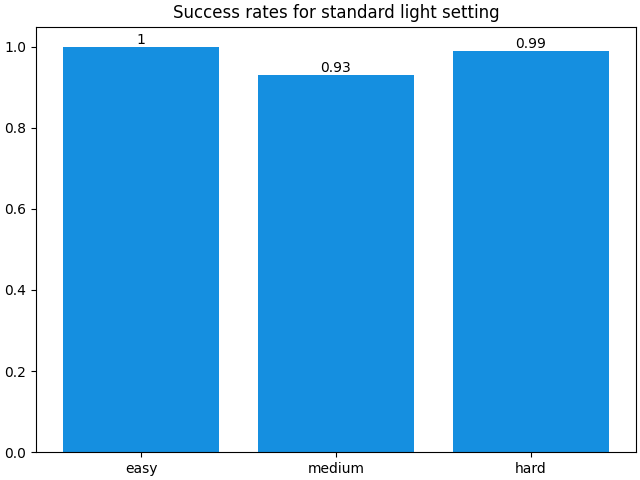
\includegraphics[width=0.45\textwidth]{Bilder/notebook_images/hardDistanceStandardLight_eval_standard_success_rates_barplot.png}
    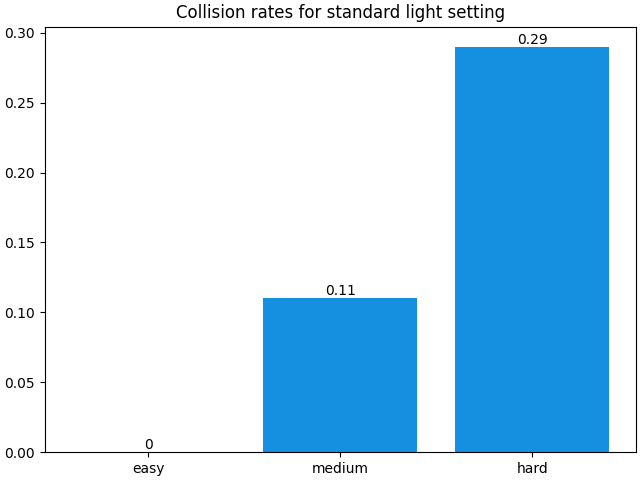
\includegraphics[width=0.45\textwidth]{Bilder/notebook_images/hardDistanceStandardLight_eval_standard_collision_rates_barplot.png}
    \caption{Success and collision rates for all difficulties for an agent trained exclusively on hard tracks with standard light}
    \label{fig:hardDistance_generalization}
\end{figure}

\paragraph{Generalization to different light settings}
\label{cha:experiment_fixed_difficulty_light_settings}

Further evaluation of these policies on different light settings showed that the policies were able to generalize to the different light settings as well. The policies were trained on the standard light setting only. However the policies were able to solve episodes with the bright and dark light settings with only slight decreases in performance. The success rates for the different light settings are shown in figure \ref{fig:hardDistance_generalization_light_settings}.

The histogram equalization preprocessing step was used during the training and evaluation of this policy. This step is mostly responsible for the good performance at different light settings \ref{sec:importance_histogram_equalization}.

\begin{figure}
    \centering
    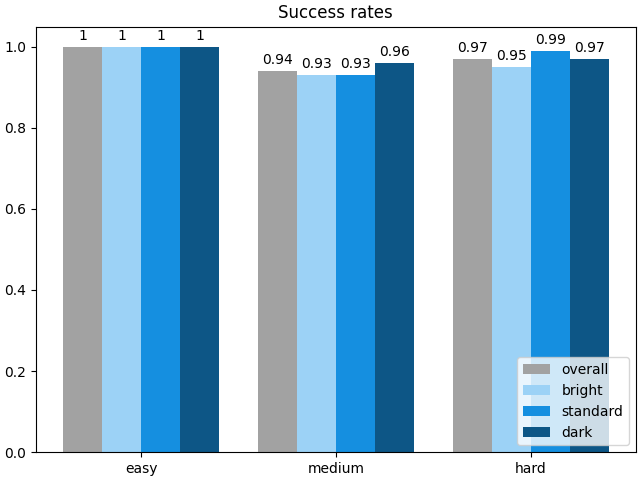
\includegraphics[width=0.45\textwidth]{Bilder/notebook_images/hardDistanceStandardLight_eval_all_success_rates_barplot.png}
    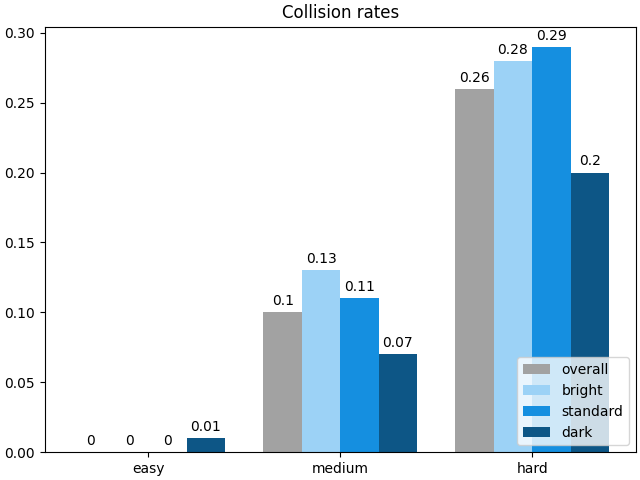
\includegraphics[width=0.45\textwidth]{Bilder/notebook_images/hardDistanceStandardLight_eval_all_collision_rates_barplot.png}
    \caption{All success and collision rates for an agent trained exclusively on hard tracks with standard light}
    \label{fig:hardDistance_generalization_light_settings}
\end{figure}

\section{Experiments training with mixed difficulty setting}
\label{cha:experiment_mixed_difficulty}

The next step was to train the policy on all difficulty levels at the same time. The goal was to find hyperparameters that would allow the policy to learn to solve all difficulty levels better than with the previous exclusive training. The policy was trained on all difficulty levels at the same time with the same hyperparameters that were used before. The $trainingMapType$ parameter was set to $randomEval$, this results in split of 20\% easy, 40\% medium and 40\% hard tracks.

The training with mixed tracks for the data collection episodes failed. The policy was not able to learn to solve the tracks as successfully as the isolated training on hard tracks. Further changes to the hyperparameters did not improve the learning process. For example the amount of data collected in each iteration was increased to balance out the increased variety of tracks.


\section{Experiments training with mixed light setting hyperparameter}
\label{cha:experiment_mixed_light}

In the previous experiments, the complexity of the task was reduced by focusing on single light settings. The goal was to test the parameters and find configurations that enable the policy to learn the tasks with increasing complexity. The experiments showed that a policy that is trained on hard tracks exclusively is able to generalize to the lower difficulty tracks as well. These policies were also able to solve the tracks of differenct light settings with only slight differences in performance.


The next step was to train the policy on all light settings at the same time. The goal was to find hyperparameters that would allow the policy to learn to solve the tracks with different light settings better than with the previous exclusive training. The policy was trained on difficult tracks with all light settings. The $lightSetting$ parameter was set to $random$, this results in split of 33\% bright, 33\% standard and 33\% dark illumination for the data collection episodes.

\paragraph{Resuts for standard light setting}

The policy was able to learn to solve the tracks of different difficulties. Similarly to the previous experiments, the policy was able to generalize to the easy and medium tracks. The policy was able to solve the easy, medium and hard tracks with success rates of 100\%, 100\% and 99\% \ref{fig:hardDistance_mixedLight_generalization}. 

This is an improvement over the policy trained exclusively on hard tracks with standard light \ref{cha:experiment_fixed_difficulty}.
This improvement may be due to the increased variety of data encountered during the training phase.

\begin{figure}
    \centering
    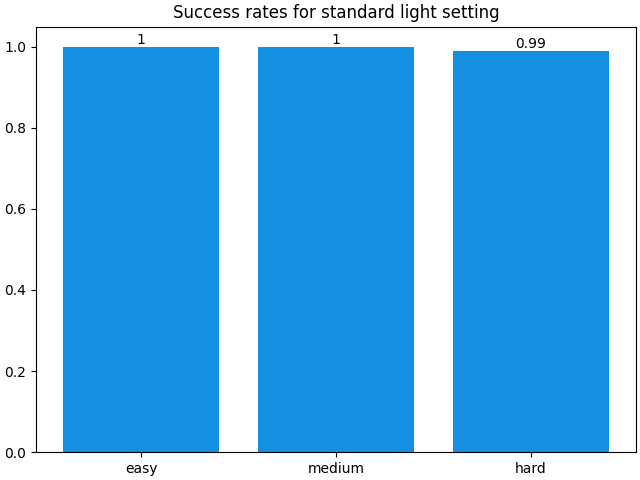
\includegraphics[width=0.45\textwidth]{Bilder/notebook_images/hardDistanceMixedLight_eval_standard_success_rates_barplot.png}
    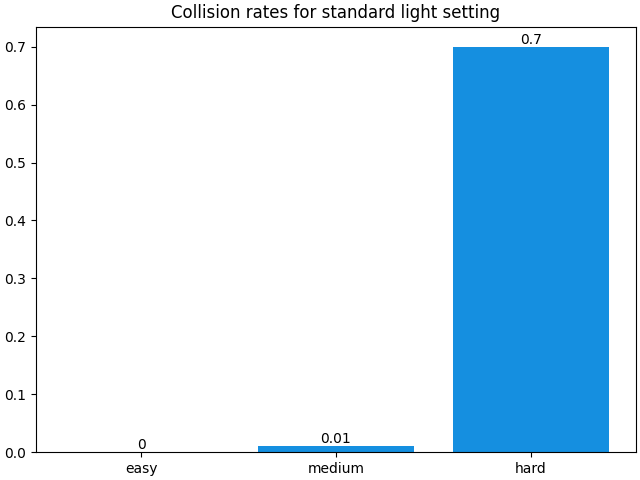
\includegraphics[width=0.45\textwidth]{Bilder/notebook_images/hardDistanceMixedLight_eval_standard_collision_rates_barplot.png}
    \caption{Success and collision rates for all difficulties with standard light for a policy trained on hard tracks with all light settings \ac{MLSP}}
    \label{fig:hardDistance_mixedLight_generalization}
\end{figure}

\paragraph{Performance on all light settings}

The policy was evaluated on the different light settings. The policy was able to solve the episodes reliably for all light settings. There were only slight differences in performance between the light settings for hard tracks \ref{fig:hardDistance_mixedLightTraining_results}.


This policy performed much better in episodes with bright or dark light setting compared to the policy trained exclusively on tracks with standard light \ref{cha:experiment_fixed_difficulty}. This was to be expected as this policy was trained on all light settings.

\begin{figure}
    \centering
    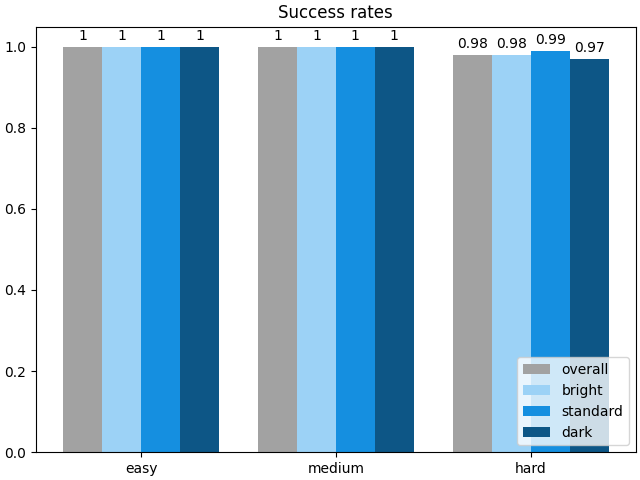
\includegraphics[width=0.45\textwidth]{Bilder/notebook_images/hardDistanceMixedLight_eval_all_success_rates_barplot.png}
    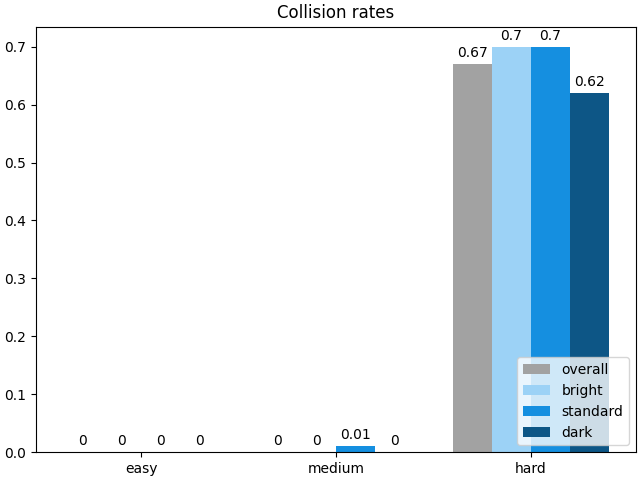
\includegraphics[width=0.45\textwidth]{Bilder/notebook_images/hardDistanceMixedLight_eval_all_collision_rates_barplot.png}
    \caption{Success and collision rates for a policy trained on hard tracks with all light settings \ac{MLSP}}
    \label{fig:hardDistance_mixedLightTraining_results}
\end{figure}



\section{Experiments on the importance of the histogram equalization preprocessing step}
\label{sec:importance_histogram_equalization}

The previous training results showed that the policy was able to learn to solve the tracks with different light settings. The histogram equalization preprocessing step was applied to the preprocessed image \ref{sec:histogram_equalization} to increase the policy's resilience towards light changes.

Policies that were trained on the standard light setting were able to solve tracks under bright and dark light conditions as well. This implies the histogram equalization plays a big role.

\paragraph{Evaluating a policy without the histogram equalization preprocessing step}

The policy from the previous section about mixed light settings during training \ac{MLSP} was trained with the histogram equalization preprocessing step. This policy was now evaluated without the histogram equalization step. 

The removal of the preprocessing step leads to a performance collapse for the standard and dark settings \ref{fig:hardDistance_mixedLight_comparison_withWithoutHistogramEqualization}. The success rate drops to 0\% for the dark light setting.
The performance for the bright light setting is not affected as severely. Nevertheless the success rate drops from 98\% to 62\% for the hard tracks.

The decrease in performance was to be expected, as the policy was trained with the histogram equalization preprocessing step. The histogram equalization step changes the image content substantially \ref{table:preprocessing_steps}. The policy has learned to use the output of the preprocessing step. As a result, the policy is not able to solve the tracks without the preprocessing step.

\begin{figure}
    \centering
    \subfigure[Success rate with histogram equalization]{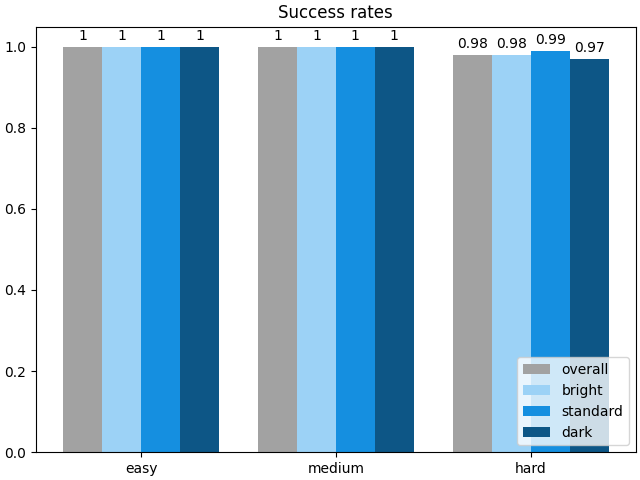
\includegraphics[width=0.45\textwidth]{Bilder/notebook_images/hardDistanceMixedLight_eval_all_success_rates_barplot.png}}
    \subfigure[Success rate without histogram equalization]{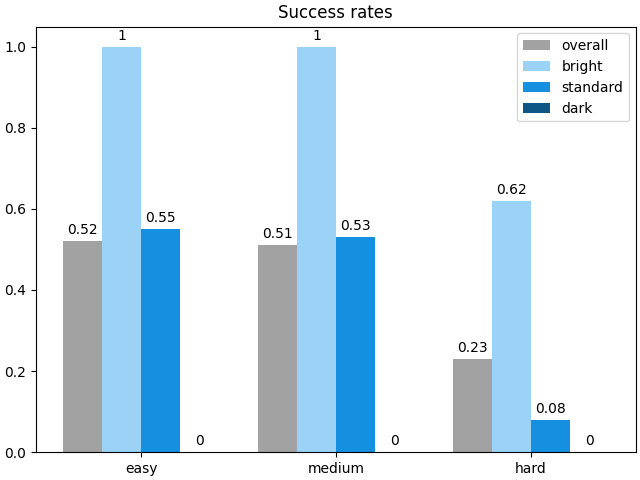
\includegraphics[width=0.45\textwidth]{Bilder/notebook_images/hardDistanceMixedLight_evalWithoutHistEqualization_all_success_rates_barplot.png}}
    \caption{Success rates for a policy trained on all light settings with histogram equalization \ac{MLSP}}
    \label{fig:hardDistance_mixedLight_comparison_withWithoutHistogramEqualization}
\end{figure}


\paragraph{Training a policy without the histogram equalization preprocessing step}
A policy without the histogram equalization preprocessing step was trained on the mixed light setting to determine if the preprocessing step is required for high performance. The results are shown in the second graph in \ref{fig:hardDistance_mixedLight_noHistogramEqualizationTraining_results}. 

The policy was not able to learn to solve the hard tracks as successfully as the policy trained with the histogram equalization preprocessing step. The performance difference is concentrated on the hard tracks.

\begin{figure}
    \centering
    \subfigure[Policy trained with histogram equalization (\ac{MLSP})]{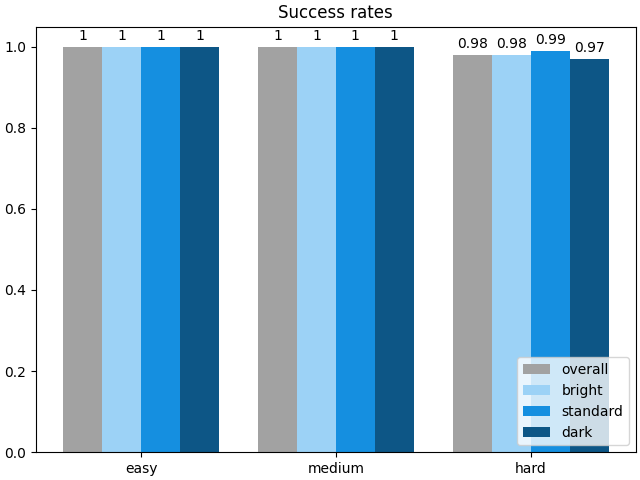
\includegraphics[width=0.45\textwidth]{Bilder/notebook_images/hardDistanceMixedLight_eval_all_success_rates_barplot.png}}
    \subfigure[Policy trained without histogram equalization (\ac{MLSP-noHist})]{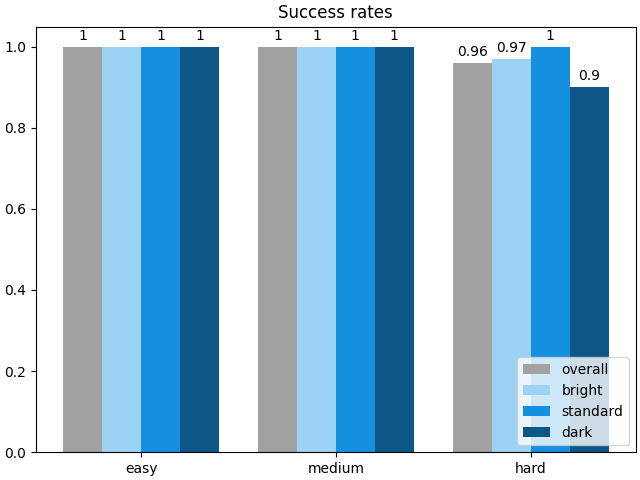
\includegraphics[width=0.45\textwidth]{Bilder/notebook_images/hardDistanceMixedLight_noHistEqualization_all_success_rates_barplot.png}}
    \caption{Success rate comparison for a policy that is trained with or without histogram equalization on all light settings}
    \label{fig:hardDistance_mixedLight_noHistogramEqualizationTraining_results}
\end{figure}


The policy \ac{MLSP-noHist} was trained without the histogram equalization preprocessing step. Adding the histogram equalization step after the training results in a decrease in performance \ref{fig:hardDistance_mixedLight_noHistogramEqualizationTraining_results_withHistogramEqualization}. 

\begin{figure}
    \centering
    \subfigure[Policy evaluation without histogram equalization]{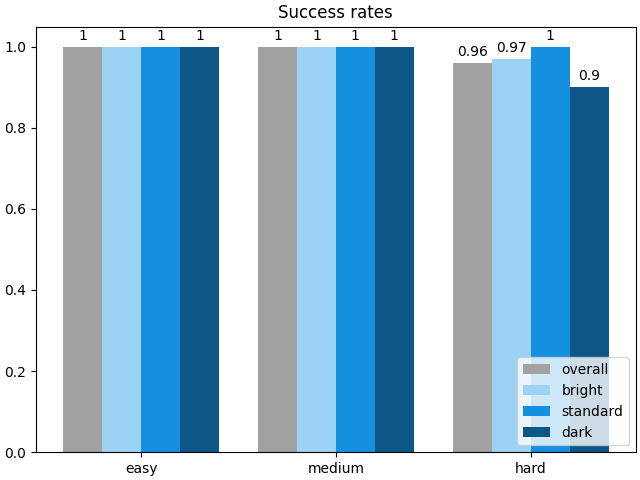
\includegraphics[width=0.45\textwidth]{Bilder/notebook_images/hardDistanceMixedLight_noHistEqualization_all_success_rates_barplot.png}}
    \subfigure[Policy evaluation with histogram equalization]{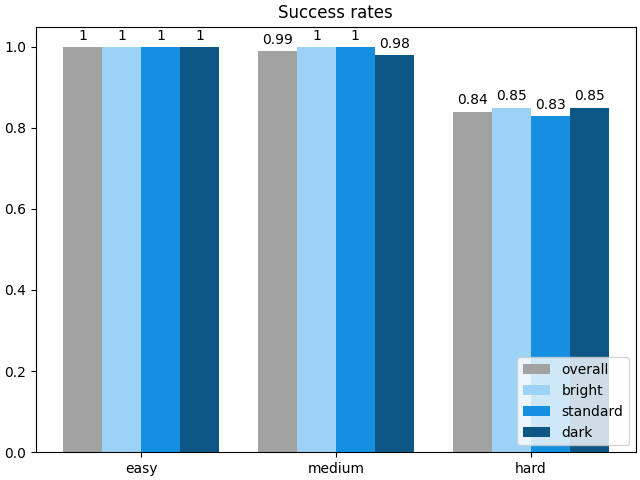
\includegraphics[width=0.45\textwidth]{Bilder/notebook_images/hardDistanceMixedLight_noHistEqualization_evalWithHistogramEqualization_all_success_rates_barplot.png}}
    \caption{Success rates for \ac{MLSP-noHist}}
    \label{fig:hardDistance_mixedLight_noHistogramEqualizationTraining_results_withHistogramEqualization}
\end{figure}


\paragraph{Conclusion}
The histogram equalization step contributes strongly to the resilience to light changes for the trained policies. It is possible to train a resilient policy without the histogram equalization preprocessing step.
However the best performance is achieved when the policy is trained with the histogram equalization preprocessing step and all light settings.

The histogram equalization preprocessing step should never be removed or added after the training is complete, this results in a performance decrease.

\section{Comment on the collision rate}
\label{sec:comment_on_collision_rate}

The trained policies are able to complete the tracks very reliably. However the policies do not avoid collisions entirely. The collision rate generally increases for higher difficulty tracks. The collision rates vary quite strongly between the different trained policies. The \ac{MLSP} policy has a collision rate of 70\% for the hard tracks with standard light setting \ref{fig:hardDistance_mixedLightTraining_results}. Whereas the \ac{SLSP} policy has a collision rate of only 29\% \ref{fig:hardDistance_generalization}.

The policies are able to complete the tracks reliably despite the collisions. The analysis of successful episodes with collisions shows that these collisions are only minor collisions. The agent collides with the goal obstacles at its side. The agent basically scapes against the goal posts. The agent does not collide with the goal obstacles head on \ref{fig:example_collision_success}.

\begin{figure}
    \centering
    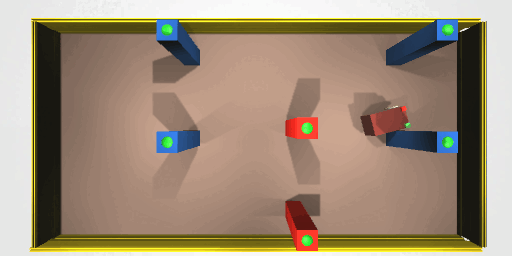
\includegraphics[width=0.45\textwidth]{Bilder/example_minor_collision_topview_frame_1295.png}
    \caption{Example of a collision from a successfully completed episode}
    \label{fig:example_collision_success}
\end{figure}

The reason for the high collision rates is the selected reward function. The policies were trained with the distance reward function exclusively following the first experimentations. The distance reward function does not penalise collisions directly. The distance reward function only discourages collisions indirectly. Collisions that prevent an agent from moving towards the next goal result in less collected reward. For example a frontal collision of the agent with a goal post object requires the agent to then move backwards and around the goal post. The backwards movement is penalized. The policy learns to avoid frontal collisions.

The minor collisions that occur are not penalized as the agent is still able to move towards the next goal. As a result the policy does not learn to avoid these collisions entirely.


\section{Hard Tracks, mixed light settings - the most successful policy \ac{MLSP}}
\label{sec:most_successful_policy}

This section summarizes how the most successful policy \ac{MLSP} was implemented and trained. The parameters were chosen following the previous experiments. This policy is used for the evaluations of the three main research goals.
The policy was trained using the distance reward alone. It was trained on hard tracks with all light settings. The policy used the histogram equalization preprocessing step.

\paragraph{Policy Settings}
The policy was configured to use the three preprocessing steps downsampling, grayscaling and histogram equalization. The policy used a frame stacking of 10. The agent camera image had a resolution of $500x168$ which was downsampled to $250x84$. This results in an observation space of shape $[84, 250, 10]$. The duration of steps was fixed to $0.3$ seconds.
The neural network follows the earlier descriptions exactly \ref{sec:network_architecture}. It consisted of a feature extractor part with 3 convolutional layers and one fully connected layer. The feature extractor takes the observation as input, its outputs are used by the action and value head. The action and value head each consist of a single fully connected layer. The entire network is trained together end-to-end using backpropagation of the loss defined by the PPO algorithm.

\paragraph{Reward function}
The policy was trained exclusively using the distance reward. The other reward functions were not used \ref{fig:final_reward_function}.

\paragraph{Training data}
The episodes for data collection used hard tracks with all light settings. The agent was initialized with random orientations. The episodes were not reset upon collision.

\paragraph{Training algorithm settings}
The training was configured to use 10 environments in parallel to collect data. 2560 samples were collected in each data collection step. The training was terminated after a total of 2385920 steps. 8423 full episodes were executed to collect these samples. 233 data collection and model training iterations were executed in total. The total training duration was 1.02 days.
The training progress can be seen in figure \ref{fig:training_most_successful_model}. The model reached a success rate of 100\% for the collected episodes.


The full training config can be found in the appendix \ref{cha:most_successful_config}.

\begin{figure}
    \centering
    \subfigure[Distance Reward]{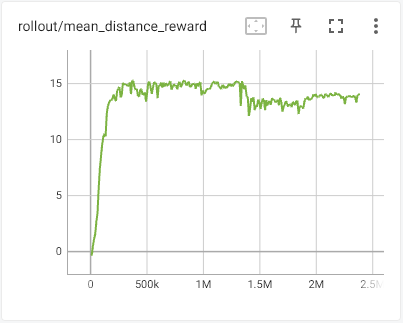
\includegraphics[width=0.3\textwidth]{Bilder/tensorboard_images/successfulTraining_distance_reward.png}}
    \subfigure[Goal completion rate]{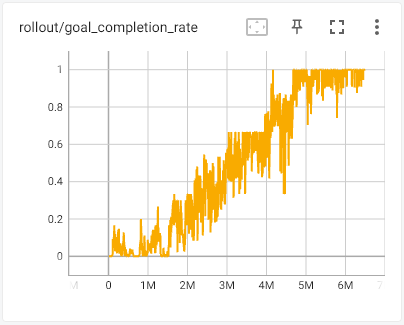
\includegraphics[width=0.3\textwidth]{Bilder/tensorboard_images/successfulTraining_goal_completion_rate.png}}
    \subfigure[Success rate]{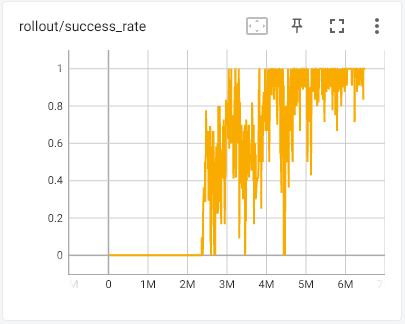
\includegraphics[width=0.3\textwidth]{Bilder/tensorboard_images/successfulTraining_success_rate.png}}
    \caption{Properties of the collected episodes over time for the most successful model}
    \label{fig:training_most_successful_model}
\end{figure}